\documentclass{beamer}

\mode<presentation> {

    \usetheme{Madrid}
    \usecolortheme{beaver}
}


\usepackage{graphicx}


%--------------------------------------------------
% Macros
%--------------------------------------------------
\newtheorem{command}[theorem]{Command}

%--------------------------------------------------
% Title Page
%--------------------------------------------------

\title[git]{A short introduction to git}
\author{John Ladan}
\institute[Waterloo]{University of Waterloo\\john@ladan.ca}
\date{\today}

\begin{document}

\begin{frame}
    \titlepage
\end{frame}

\begin{frame}
    \frametitle{Overview}
    \tableofcontents
\end{frame}

%--------------------------------------------------
% Presentation slides
%--------------------------------------------------

\section{What is git?}

\begin{frame}
    \frametitle{According to git-scm.com}
    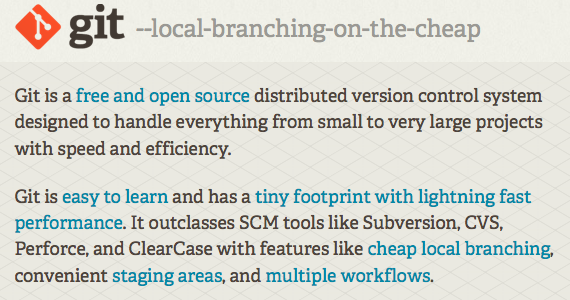
\includegraphics{figures/git-homepage}
\end{frame}

\begin{frame}
    \frametitle{According to wikipedia.org}
    Git (/ɡɪt/) is a distributed revision control system with an emphasis on speed, data integrity, and support for distributed, non-linear workflows. Git was initially designed and developed by Linus Torvalds for Linux kernel development in 2005, and has since become the most widely adopted version control system for software development.

    As with most other distributed revision control systems, and unlike most client–server systems, every Git working directory is a full-fledged repository with complete history and full version-tracking capabilities, independent of network access or a central server. Like the Linux kernel, Git is free software distributed under the terms of the GNU General Public License version 2.
\end{frame}

\begin{frame}
    \frametitle{Features}
    \begin{itemize}
        \item Fast
        \item Nonlinear development (via rapid branching, and DAG based structure)
        \item Distributed -- each copy of the repo is complete by itself
            \begin{itemize}
                \item each copy of the repo is itself a repo
                \item changes can be pushed/pulled to any other instance
                \item do not need network access
            \end{itemize}
        \item Ubiquitous
        \item Good \em{free} repository hosting (github)
    \end{itemize}
\end{frame}

\section{Cloning a Repo}

\begin{frame}
    \frametitle{Git Clone}
    \begin{command}
        \texttt{git clone <repository-location> [<local-path>]}
    \end{command}
    It's a lot like downloading a tarball, except
    \begin{itemize}
        \item only the necessary files are included (no build files)
        \item lots of option, like pulling a specific commit, or not downloading full history
    \end{itemize}
\end{frame}

\begin{frame}
    \frametitle{Submodules}
    Word of warning: some packages use \em{submodules}. One way to handle it:
    \begin{command}
        \texttt{git clone --recursive <repo>}
    \end{command}
\end{frame}

\section{Making Changes}

\begin{frame}
    \frametitle{Branching}
    You should always branch first:
    \pause
    \begin{itemize}
        \item it's a good habit to be in;
        \item the last good state is left labeled;
        \item easy to checkout other branches, even when you're in the middle of something;
        \item pulling origin/master is easier; and
        \item branches are cheap!
    \end{itemize}
\end{frame}

\begin{frame}
    \frametitle{Git Branch}
    \begin{command}
        \texttt{git branch <branch-name>}\\
        \texttt{git checkout <branch-name>}
    \end{command}
    Alternatively,
    \begin{command}
        \texttt{git checkout -b <branch-name>}
    \end{command}
\end{frame}


\begin{frame}
    \frametitle{Editing}
    When editing, you can use whatever tools you want, with one (or two) exceptions:
    \pause
    moving and removing files.
    \begin{command}
        \texttt{git mv <file> <new-filename>}
    \end{command}
    \begin{command}
        \texttt{git rm <file>}
    \end{command}
    This way, git understands that it is the same file (or that it is intentionally gone).
\end{frame}


\section{Commiting Changes}

\begin{frame}
    \frametitle{Seeing your changes}
    First, it's a good idea to see what changes you made
    \begin{command}
        \texttt{git status}
    \end{command}
    \pause
    And if you want the details,
    \begin{command}
        \texttt{git diff <file>}
    \end{command}
\end{frame}

\begin{frame}
    \frametitle{Staging files}
    Next, we need to let git know what files have changed, and what new files it should track
    \begin{command}
        \texttt{git add <file(s)>}
    \end{command}
    \pause
    Often, it's good to check the \em{status} again before the next step
\end{frame}

\begin{frame}
    \frametitle{Commit!}
    Finally, we commit our changes to the tree.
    \begin{command}
        \texttt{git commit [-m "Message text"]}
    \end{command}
    \pause
    (I recommend not using the \texttt{-m} flag)
\end{frame}


\begin{frame}
    \frametitle{Practice safe committing}
    Here are a few best practices:
    \begin{itemize}
        \item Commits should be small and non-breaking
        \item The message should complete the sentence ``This commit will...''
        \item Keep the commit to one feature/bug-fix
        \item Don't use the \texttt{-m} flag
    \end{itemize}
\end{frame}

\begin{frame}
    \frametitle{Speeding up commits}
    There's a faster way...
    \begin{command}
        \texttt{git commit -a}
    \end{command}
    The \texttt{-a} flag stages \em{all} modified files, but not any untracked files.
\end{frame}

\section{Rolling Your Own}

\begin{frame}
    \frametitle{Typical Case}
    This is what often happens...
    \begin{itemize}
        \item start coding, and realize you want this in a git repo
        \item create a new repo
    \end{itemize}
    \begin{command}
        \texttt{git init ; git add... ; git commit}
    \end{command}
    \begin{itemize}
        \item continue coding, then realize you want a remote backup
        \item create a repo on github, then...
    \end{itemize}
    \begin{command}
        \texttt{git remote add origin <repo-url>; git push -u master origin}
    \end{command}
\end{frame}


\begin{frame}
    \frametitle{Problems}
    Pros:
    \begin{itemize}
        \item you can always retroactively add version control to a project
    \end{itemize}
    Cons:
    \begin{itemize}
        \item All the past revision history is lost.
        \item These commands are more obscure and harder to remember.
    \end{itemize}
\end{frame}

\begin{frame}
    \frametitle{Ideal Case}
    \begin{itemize}
        \item Have the foresight to create a repo (e.g. on github)
        \item Clone that repo onto your workstation
        \item Start coding and commiting as usual
    \end{itemize}
\end{frame}


\begin{frame}
    \frametitle{One more thing}
    If you don't want to share your project publicly, and have access to a server,
    \begin{command}
        \texttt{git init --bare}
    \end{command}
    This creates a "headless" repo, storing all the data, but without the working tree. You can then push/pull/clone from this remote repo as usual.
    \pause

    E.g. I put all of my repos in a directory on CSC servers. \texttt{jladan@taurine.uwaterloo.ca:/users/jladan/git-repos/}
\end{frame}

\section{Version Control}

% What's this HEAD thing, and all those numbers? (commit hash)
% Tagging
% master branch
% undoing changes that haven't been committed
% going back a bit further (HEAD~1)

\section{In Practice}

% - `git status` will tell you most of what you need (it suggests commands)
% - create an alias for glog
% - search for how to do things on google
% - forking and pull requests
% - github
% - git stash & git stash pop (made changes but forgot to branch)
% - for your own project, it should be more linear
% - delete your old branches (after they're merged back in)
% - `git commit --amend` to fix that last commit

\end{document}
